\chapter{Implementación}

En este capítulo se hablará del desarrollo del software describiendo la plataforma de desarrollo y despliegue, así como las distintas decisiones tomadas a la hora de implementar y las fases de desarrollo.

\section{Plataforma de desarrollo}

En un principio, la idea fue desarrollar usando una distribución Linux un \textbf{software multiplataforma} ayudándose, para ello, de CMake \cite{cmake} que a partir de los archivos fuentes puede crear \textit{makefiles} para distintas plataformas.

No obstante, unos problemas detectados con los \textit{drivers} de mi GPU provocaban que no se pudiese integrar Qt \cite{qt} con VTK \cite{vtk} ya que el \textit{widget} especializado para esta tarea (\texttt{QVTKWidget}) no funcionaba. Tras unos días intentando solucionar los problemas sin éxito se decidió migrar a Windows donde no surgió ningún problema parecido al que se dio en Linux.

Más tarde además de Qt y VTK se decidió utilizar la librería Boost \cite{boost} para facilitar el tratamiento de ficheros XML.

Se ha utilizado \textbf{Windows 10 Pro} (64 bits) con el siguiente software y librerías:

\begin{itemize}
	\item CMake 3.4.1
	\item Visual Studio Community 2013
	\item Qt5.5.1
	\item VTK 7.0.0
	\item Boost 1.60.0
\end{itemize}

Cuando se empezó a desarrollar el software la versión más nueva de VTK era la \textbf{6.3.0} y se empezó utilizando ésta. No obstante, tenía un pequeño fallo que afectaba mucho a la aplicación y es que si se hacía uso de la GPU en el \textit{ray casting} al renderizar el volumen, \textbf{la opacidad gradiente no se computaba}. Por suerte, a principios del mes de Febrero, se lanzó una nueva versión de VTK, la \textbf{7.0.0}, que solucionaba este fallo.

Pero los problemas no acababan aquí, y es que, con la nueva versión, el programa no llegaba a funcionar y \textbf{se bloqueaba nada más iniciarse}. Detectar el fallo era complicado y al no ser todavía demasiado complejo era más rápido detectar de dónde venía el error si se volvía a crear desde cero agregando uno a uno cada componente.

\textbf{El fallo lo estaba dando el plano de corte} y es que en la versión anterior al activarlo, si no tenía ningún volumen con el que cortar, no producía ningún fallo, pero con la nueva versión era un requisito imprescindible. La solución era bastante sencilla: habilitar el plano cuando se cargase el volumen en lugar de tenerlo habilitado desde su propia construcción.

\section{Instalación y configuración}

\subsection{Entorno de desarrollo}

\subsubsection{Visual Studio Community 2013}

\begin{itemize}
	\item Descargar Visual Studio Community 2013 desde su \href{https://www.visualstudio.com/es-es/downloads/download-visual-studio-vs.aspx}{web oficial} e instalar.
\end{itemize}

\subsubsection{Qt5.5.1}

\begin{itemize}
	\item Descargar Qt5.5.1 desde \href{http://download.qt.io/official_releases/qt/5.5/5.5.1/qt-opensource-windows-x86-msvc2013-5.5.1.exe}{este enlace} de su web e instalar.
	\item Crear una nueva variable de entorno con nombre \texttt{QTDIR} y valor \texttt{C:\textbackslash\\ Qt\textbackslash Qt5.5.1} (directorio raíz de la versión instalada).
	\item Agregar al PATH la siguiente dirección \texttt{C:\textbackslash Qt\textbackslash Qt5.5.1\textbackslash 5.5\textbackslash msvc2013\\ \textbackslash bin}.
\end{itemize}

\subsubsection{CMake 3.4.1}

\begin{itemize}
	\item Descargar CMake 3.4.1 desde \href{https://cmake.org/files/v3.4/cmake-3.4.1-win32-x86.exe}{este enlace} de su web e instalar (al instalar se recomienda marcar la opción de agregar al PATH de todos los usuarios para no tener que hacerlo manualmente).
\end{itemize}

\subsection{Compilar librerías}

\subsubsection{VTK 7.0.0}

\begin{itemize}
	\item Descargar VTK 7.0.0 desde \href{http://www.vtk.org/files/release/7.0/VTK-7.0.0.zip}{este enlace} de su web oficial y extraer en \texttt{C:\textbackslash VTK\textbackslash 7.0.0\textbackslash src}.
	\item Abrir CMake y completar:
	\begin{itemize}
		\item src: \texttt{C:\textbackslash VTK\textbackslash 7.0.0\textbackslash src}
		\item build: \texttt{C:\textbackslash VTK\textbackslash 7.0.0\textbackslash build\textbackslash vs12}
	\end{itemize}
	\item Elegir como generador \textit{Visual Studio 12 2013}.
	\item Presionar configurar.
	\item Una vez generado seleccionar los siguientes campos:
	\begin{itemize}
		\item \texttt{BUILD\_SHARED\_LIBS}
		\item \texttt{Module\_vtkGUISupportQt}
		\item \texttt{Module\_vtkGUISupportQtOpenGL}
		\item \texttt{Module\_vtkGUISupportQtSQL}
		\item \texttt{Module\_vtkGUISupportQtWebkit}
		\item \texttt{Module\_vtkRenderingQt}
		\item \texttt{Module\_vtkViewsQt}
		\item \texttt{Module\_vtkDICOM}
		\item \texttt{VTK\_Group\_Qt}
	\end{itemize}
	\item Agregar dos entradas:
	\begin{itemize}
		\item \texttt{QT\_QMAKE\_EXECUTABLE:PATHFILE=\\C:\textbackslash Qt\textbackslash Qt5.5.1\textbackslash 5.5\textbackslash msvc2013\textbackslash bin\textbackslash qmake.exe}
		\item \texttt{CMAKE\_PREFIX\_PATH:PATH=C:\textbackslash Qt\textbackslash Qt5.5.1\textbackslash 5.5\textbackslash msvc2013\textbackslash}
	\end{itemize}
	\item Presionar en configurar y aparecerá un error, habrá que elegir como versión de Qt la 5. Elegirla y volver a configurar.
	\item Configurar hasta que no aparezca ningún campo en rojo.
	\item Una vez configurado todo, pulsar en generar. Esto creará una serie de archivos en \texttt{C:\textbackslash VTK\textbackslash 7.0.0\textbackslash build\textbackslash vs12}.
	\item Abrir \texttt{VTK.sln}.
	\item Construir en modo \textit{Release} y esperar unos minutos a que termine.
	\item Copiar los archivos \texttt{QVTKWidgetPlugin.lib} y \texttt{QVTKWidgetPlugin.dll} que se encuentran en \texttt{C:\textbackslash VTK\textbackslash 7.0.0\textbackslash build\textbackslash vs12\textbackslash lib\textbackslash Release} y \texttt{C:\textbackslash\\  VTK\textbackslash 7.0.0\textbackslash build\textbackslash vs12\textbackslash bin\textbackslash Release} respectivamente en \texttt{C:\textbackslash Qt\textbackslash\\ Qt5.5.1\textbackslash 5.5\textbackslash msvc2013\textbackslash plugins\textbackslash designer} (Si no se encuentran los archivos, comprobar que en CMake se marcó la opción \texttt{BUILD\_SHARED\_\\ LIBS}). Esto hará que desde Qt Designer se pueda crea un \texttt{QVTKWidget}.
	\item Construir en modo \textit{Debug}.
	\item Crear una nueva variable de entorno con nombre: \texttt{VTK\_DIR} y valor: \texttt{C:\textbackslash VTK\textbackslash 7.0.0\textbackslash build\textbackslash vs12}.
	\item Agregar al Path la siguiente dirección: \texttt{C:\textbackslash VTK\textbackslash 7.0.0\textbackslash build\textbackslash vs12\textbackslash bin\\ \textbackslash Release}.
\end{itemize}

\subsubsection{Boost 1.60.0}

\begin{itemize}
	\item Descargar Boost 1.60.0 desde \href{http://sourceforge.net/projects/boost/files/boost/1.60.0/}{este enlace} de su web oficial.
	\item Descomprimir en cualquier lugar, abrir la consola de comandos de Visual Studio y moverse al lugar donde ha sido extraído.
	\item Escribir \texttt{boostrap.bat} para generar el \texttt{Boost.Build}.
	\item Compilar con: \texttt{b2 toolset=msvc-12.0 --build-type=complete \\ --abbreviate-paths architecture=x86 address-model=64 \\ install -j4}.
	\item Agregar al proyecto de Visual Studio: 
\end{itemize}

\subsection{Configurar proyecto}

Una vez generado el proyecto realizar los siguientes cambios en la configuración: 
\begin{itemize}
	\item En \textit{Project Properties} ir a \textit{Configuration Properties $ \rangle $ C/C++ $ \rangle $ General $ \rangle $ Additional Include Directories} y añadir el directorio \texttt{C:\textbackslash Boost\textbackslash \\  include\textbackslash boost-1\_60}.
	\item En \textit{Project Properties} ir a \textit{Configuration Properties $ \rangle $ Linker $ \rangle $ Additional Library Directories} y añadir el directorio \texttt{C:\textbackslash Boost\textbackslash lib}.
	\item En \textit{Project Properties} ir a \textit{Configuration Properties $ \rangle $ Linker $ \rangle $ System} y:
	\begin{itemize}
		\item En \textit{Subsystem} seleccionar la opción: \\ \texttt{Windows (/SUBSYSTEM:WINDOWS)}.
		\item En \textit{Enable Large Adresses} seleccionar la opción: \\ \texttt{Yes (/LARGEADRESSESAWARE)}.
	\end{itemize}
\end{itemize}

\section{Conceptos clave en Volume Rendering}

\subsection{Técnicas de renderizado}

A la hora de renderizar un conjunto de datos volumétricos para obtener una imagen en 3D, se pueden utilizar distintas técnicas y VTK proporciona una serie de clases para su uso:

\begin{itemize}
	\item \textbf{\textit{Marching cubes}}: Con este algoritmo se obtiene una malla poligonal de una isosuperficie a partir de un conjunto de datos volumétrico (Figura \ref{fig:marching_cubes_head}) \cite{marching_cubes}. Se puede usar en VTK con \texttt{vtkMarchingCubes}.
	\begin{figure}[H]
		\centering
		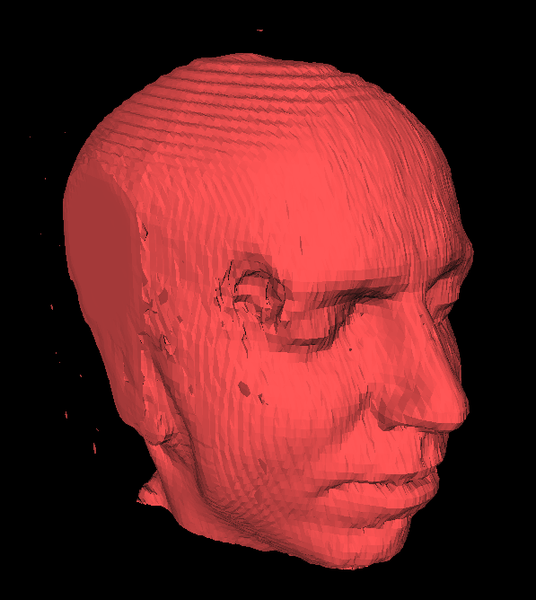
\includegraphics[width=6cm]{imagenes/marching_cubes_head}
		\caption{Cabeza extraída de 150 cortes obtenidos por una IRM usando \textit{marching cubes} (sobre 150.000 triángulos). Imagen extraída de \url{https://en.wikipedia.org/wiki/File:Marchingcubes-head.png}}
		\label{fig:marching_cubes_head}
	\end{figure}
	
	\item \textbf{Texturas 2D}: Se utilizan planos de corte alineados a los ejes de coordenadas. Por lo que se tendría una serie de cortes sobre el plano sagital, otra sobre el coronal y otra sobre el axial. Se realiza una interpolación bilineal para obtener la imagen final (Figura \ref{fig:texturas2d} \cite{intro_medical_vtk_bioimage}). Se puede usar en VTK con \texttt{vtkVolumeTextureMapper}.
	\begin{figure}[H]
		\centering
		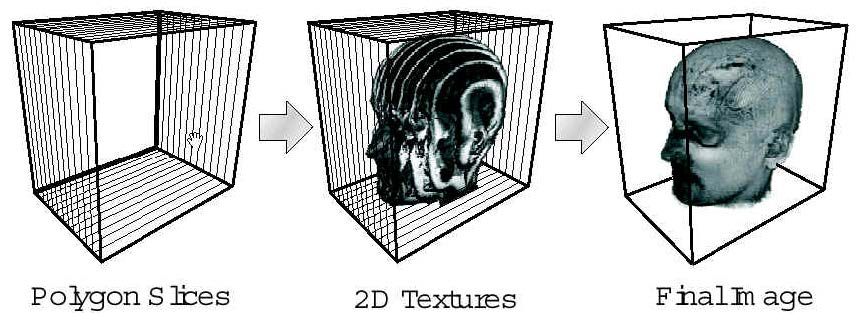
\includegraphics[width=10cm]{imagenes/texturas2d}
		\caption{Esquema del proceso de renderizado usando texturas 2D. Imagen extraída del apéndice B del libro \textit{An Introduction to Programming for Medical Image Analysis with the Visualization Toolkit} \cite{intro_medical_vtk_bioimage}}
		\label{fig:texturas2d}
	\end{figure}
	
	\item \textbf{Texturas 3D}: Esta técnica es similar a la anterior, pero ahora los datos se cargan en una textura 3D y los cortes se dibujan paralelos a la dirección de vista. A diferencia de las texturas 2D, usa interpolación trilineal y no es necesario tener almacenado en memoria tres copias de los mismos datos (Figura \ref{fig:texturas3d}) \cite{intro_medical_vtk_bioimage}. Se puede usar en VTK con \texttt{vtkVolumeTextureMapper3D}.
	\begin{figure}[H]
		\centering
		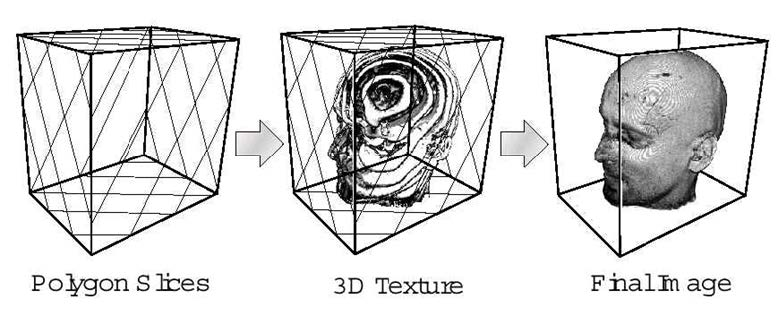
\includegraphics[width=10cm]{imagenes/texturas3d}
		\caption{Esquema del proceso de renderizado usando texturas 3D. Imagen extraída del apéndice B del libro \textit{An Introduction to Programming for Medical Image Analysis with the Visualization Toolkit} \cite{intro_medical_vtk_bioimage}}
		\label{fig:texturas3d}
	\end{figure}
	
	\item \textbf{\textit{Ray casting}}: Es una técnica en la que para cada pixel de la imagen se lanza un rayo que atraviesa el volumen. Para cada voxel se obtiene su color y opacidad usando una función de transferencia. Cuando el rayo sale del volumen se calcula el color y opacidad del pixel como el acumulado por el rayo. Existe una versión de este algoritmo que hace uso de la GPU para acelerar ostensiblemente el tiempo de la operación (Figura \ref{fig:volume_ray_casting}) \cite{intro_medical_vtk_bioimage}. Se puede usar en VTK con \texttt{vtkFixedVolumeRayCastMapper}, \texttt{vtkVolumeRayCastMapper} (usan CPU), \texttt{vtkGPUVolumeRayCastMapper} (usa GPU) y \texttt{vtkSmartVolumeMapper} (según el contexto usa CPU o GPU).
	\begin{figure}[H]
		\centering
		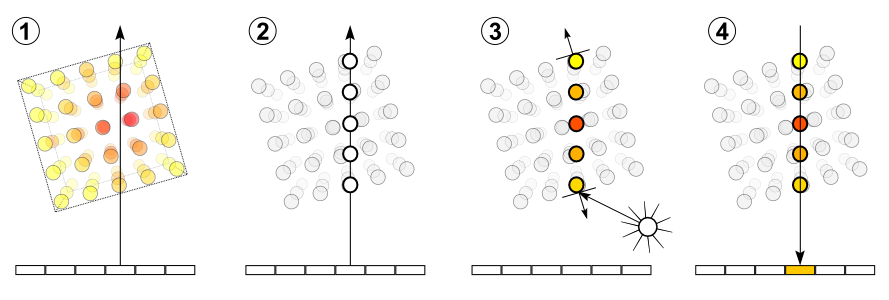
\includegraphics[width=12.5cm]{imagenes/volume_ray_casting}
		\caption{Esquema del proceso de \textit{ray casting}. Imagen extraída de \url{https://en.wikipedia.org/wiki/File:Volume_ray_casting.png}}
		\label{fig:volume_ray_casting}
	\end{figure}
\end{itemize}

De entre todas estas técnicas, se podrían descartar rápidamente la de \textit{marching cubes}: pues tan solo trabaja con isosuperficies, y la de texturas 2D: pues la opción de texturas 3D es más rápida y usa menos recursos. Sin embargo, la opción de \textit{marching cubes} será útil para poder crear una malla de triángulos que se pueda exportar a un formato con el que luego pueda ser imprimida en 3D.

Por tanto ya solo habría que elegir entre texturas 3D o \textit{ray casting}. Hasta hace unos años, VTK no proporcionaba un algoritmo de \textit{ray casting} que usase la GPU. Por tanto la opción habría sido sencilla, pero durante los últimos años han trabajado en esto haciendo del \textit{ray casting} la opción preferible.

\subsection{Volume Mapper}

Para poder visualizar un volumen con VTK mediante Direct Volume Rendering (DVR), necesitamos un \textit{Volume Mapper}. La librería nos ofrece varias alternativas:

\begin{itemize}
	\item \texttt{vtkAMRVolumeMapper}
	\item \texttt{vtkFixedVolumeRayCastMapper}
	\item \texttt{vtkGPUVolumeRayCastMapper}
	\item \texttt{vtkSmartVolumeMapper}
	\item \texttt{vtkVolumeRayCastMapper}
	\item \texttt{vtkVolumeTextureMapper}
	\item \texttt{vtkVolumeTextureMapper3D}
\end{itemize}

Entre esta lista tenemos algunos que utilizan o texturas o \textit{ray casting}, o la CPU o la GPU. Pero hay uno que es especial con respecto al resto. Se trata de \texttt{vtkSmartVolumeMapper}.

Este \textit{Volume Mapper} es una versión mejorada del \texttt{vtkGPUVolumeRayCast Mapper} por lo que utiliza la GPU (si el dispositivo cuenta con una) y la técnica de \textit{ray casting}. Además cuenta con nuevas características con respecto al resto, como el poder definir infinitos planos de corte para poder ver el interior del volumen \cite{smart_volume_mapper}.

Por tanto, el \textit{Volume Mapper} utilizado será el \texttt{vtkSmartVolumeMapper}.

\subsection{Función de transferencia}

La función de transferencia es la encargada de dar a un valor de intensidad las propiedades de color y opacidad que le corresponden para la visualización del volumen.

En VTK la función de transferencia forma parte de la clase \texttt{vtkVolume Property} \cite{vtk_example_medical4}. Para ello proporciona otras dos clases:

\begin{itemize}
	\item \texttt{vtkColorTransferFunction}: Para definir el color. Se enlaza a \texttt{vtk VolumeProperty} con el método \texttt{SetColor}.
	\item \texttt{vtkPiecewiseFunction}: Para definir la opacidad (tanto escalar como gradiente). La opacidad escalar se enlaza a \texttt{vtkVolumeProperty} con el método \texttt{SetScalarOpacity} y la gradiente con \texttt{SetGradientOpacity}.
\end{itemize}

Podemos, por tanto, diferenciar tres partes fundamentales en la función de transferencia, la encargada de dar la propiedad de color y las dos de dar la propiedad de opacidad. Ambas trabajan de forma independiente. Es decir, cuando se define un punto en una de ellas, no tiene por qué definirse en la otra.

\subsubsection{Color}

Para definir esta función (\texttt{vtkColorTransferFunction}), hay que agregar puntos para valores de intensidad a los que se les asignará un color. VTK se encargará de interpolar entre un punto y otro (Figura \ref{fig:color_tf}). 

Por defecto, cuando no hay ningún punto, a todos los valores de intensidad les corresponderá un color negro. De forma parecida se comporta cuando solo hay un punto pero en lugar de negro, les corresponderá el color del punto que se ha definido.

VTK permite trabajar tanto con HSV como con RGB y para añadir un punto hay que utilizar \texttt{AddHSVPoint} o \texttt{AddRGBPoint}. A estos métodos se les pasa un primer parámetro en coma flotante con el valor de intensidad donde se establecerá ese punto y otros tres con las distintas exponentes (\textit{hue}, \textit{saturation}, \textit{brightness} o \textit{red}, \textit{green}, \textit{blue}).

\begin{figure}[H]
	\centering
	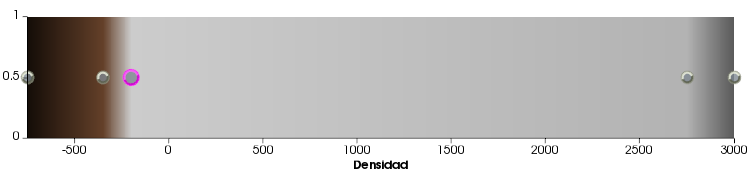
\includegraphics[width=12.5cm]{imagenes/color_tf}
	\caption{Parte de color de la función de transferencia del \textit{preset} \textit{CT-WoodSculpture} creado para visualizar esculturas de madera policromadas. Dos puntos definen el color. Uno en -750 con un tono más oscuro y otro en -350 con un tono más claro. El estuco se pinta con un color gris claro y también viene definido por dos puntos: -200 y 2750. Finalmente, el metal se verá con un tono gris oscuro definido con un punto en 3000.}
	\label{fig:color_tf}
\end{figure}

\subsubsection{Opacidad}

El valor de opacidad se obtendría como el \textbf{producto de la opacidad escalar por la gradiente}. Si no se define alguna de las dos, se definiría como un valor constante de 1 para que solo se viese el resultado de la que sí está definida.

\paragraph{\textbf{Opacidad escalar:}} Con el color no bastaría, pues si comprobásemos ahora añadiéndole tan solo el \texttt{vtkColorTransferFunction} al \texttt{vtkVolumeProperty} observaríamos que no se pinta nada en pantalla. Esto es porque por defecto, al no tener ningún punto la función de opacidad (\texttt{vtkPiecewiseFunction}) es una constante con valor 0 (transparente). 

Para definir esta función se trabaja de forma parecida a como se hace con el color, añadiendo puntos. El método que hay que utilizar es \texttt{AddPoint} al que se le pasan dos parámetros en coma flotante. El primero con el valor de intensidad y el segundo con la opacidad en ese punto. Para obtener los valores en puntos intermedios, se interpola entre los dos puntos en los que está. De forma que si para el valor de intensidad 100 hemos definido una opacidad de 0.5 y para el de 200 1, al valor de intensidad 150 le corresponderá 0.75.

Combinando color y opacidad escalar podemos obtener una función de transferencia para visualizar nuestro volumen (Figura \ref{fig:opacity_tf}), pero para obtener mejores resultados, habrá que utilizar la opacidad gradiente. 

\begin{figure}[H]
	\centering
	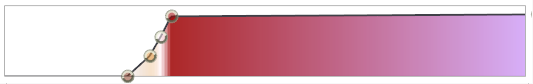
\includegraphics[width=12.5cm]{imagenes/opacity_tf}
	\caption{Parte de opacidad escalar de la función de transferencia del \textit{preset} \textit{CT-WoodSculpture} creado para visualizar esculturas de madera policromadas. Se pueden observar tres regiones. La primera corresponde a la madera, la segunda al estuco y la última al metal}
	\label{fig:opacity_tf}
\end{figure}

\paragraph{\textbf{Opacidad gradiente:}} La opacidad gradiente utiliza el vector gradiente para dar el valor de opacidad. Con éste se puede conseguir \textbf{dar un mayor valor a regiones de los bordes, así como menor a regiones planas} es decir, donde no varía el valor de intensidad de sus vecinos de alrededor.

El gradiente se mide como la cantidad que varía la intensidad en una unidad de distancia. Este cálculo del gradiente lo realiza VTK cuando genera el volumen de forma transparente sin que haya que añadir nada al código.

Para poder definir la función de la opacidad gradiente, al igual que con las demás, hay que añadir puntos con la misma función que se usaba con la opacidad escalar (\texttt{AddPoint}). 

\begin{figure}[H]
	\centering
	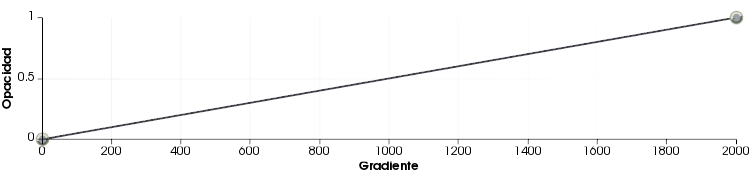
\includegraphics[width=12.5cm]{imagenes/gradient_tf}
	\caption{Parte de opacidad gradiente de la función de transferencia del \textit{preset} \textit{CT-WoodSculpture} creado para visualizar esculturas de madera policromadas. Se obtendría un valor cercano a 1 en la opacidad en aquellas zonas más cercanas a los bordes entre materiales pues se ha establecido que para un gradiente 0 la opacidad sea 0, y para 2000, 1. }
	\label{fig:gradient_tf}
\end{figure}

\subsection{Escala Hounsfield}

Como ya se ha explicado, para desarrollar la función de transferencia con la que se visualiza el volumen, juega un papel muy importante el valor de densidad del material. 

Este valor se encuentra en unas unidades conocidas como Unidades Hounsfield (HU) en honor al ingeniero Godfrey Newbold Hounsfield, inventor del primer escáner TAC con el que ganó el Premio Nobel de Fisiología o Medicina en 1979.

La Escala Hounsfield no es más que la transformación de la escala de coeficientes de atenuación lineal de rayos X a una nueva en relación al valor del agua destilada en condiciones normales de presión y temperatura.

El valor de HU de un material viene dado por la siguiente fórmula:

\[ HU = 1000 \times \frac{\mu_{mat}-\mu_{agua}}{\mu_{agua}} \]

Donde $ \mu_{mat} $ es el coeficiente de atenuación lineal del material y $ \mu_{agua} $ el del agua.

Por tanto, el valor teórico del agua será 0 HU.

El rango de valores de la escala va desde -1024 HU hasta 3071 HU. 4096 valores representados mediante 12 bits.

\begin{table}[H]
	\begin{center}
		\begin{tabular} {l|c}
			\hline
			Material & HU \\ \noalign{\hrule height 1pt}
			Aire & -1000 \\ \hline
			Madera & -750 a -350 \\ \hline
			Estuco & 200 a 1000 \\ \hline
			Metal & 2900 a 3000 \\ \hline
		\end{tabular}
		\caption{Valores en HU de distintos materiales presentes en imágenes de esculturas de madera}
		\label{tab:materials_hu}
	\end{center}
\end{table}

\section{Fases de desarrollo}

Al seguirse un desarrollo evolutivo basado en un prototipo funcional, se ha ido creando poco a poco y añadiendo componentes conforme se iban completando y probando lo que ya se había desarrollado:

\subsection{Lectura de imágenes DICOM}

El primer paso fue poder \textbf{leer una imagen DICOM}. Para ello, se utilizó el ejemplo \href{http://www.vtk.org/Wiki/VTK/Examples/Cxx/IO/ReadDICOM}{ReadDICOM} de la web de ejemplos de VTK que hace uso de \texttt{vtkDICOMImageReader} para leer la imagen.

A continuación, se pasó a \textbf{leer una serie de imágenes}. En la lista de ejemplos de VTK también había uno que realizaba esta operación: \href{http://www.vtk.org/Wiki/VTK/Examples/Cxx/IO/ReadDICOMSeries}{ReadDICOMSeries}, pero era hora de integrarlo con Qt. Y aquí es donde surgió el problema comentado anteriormente con los \textit{drivers} de la GPU.

Tras migrar a Windows y lograr crear un \textbf{pequeño programa en Qt} (Figura \ref{fig:read_dicom_series_qt}) con el que visualizar una serie de imágenes (desplazándose entre ellas con un slider) pasé a la siguiente fase, una de las más importantes, la de la reconstrucción volumétrica.

\begin{figure}[H]
	\centering
	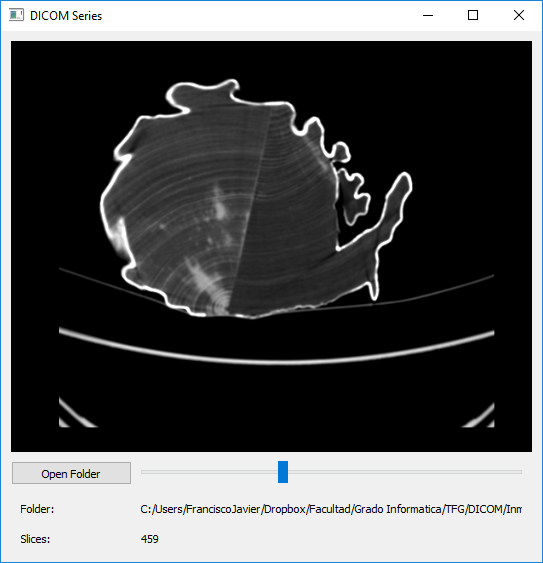
\includegraphics[width=10cm]{imagenes/read_dicom_series_qt}
	\caption{Programa sencillo para visualizar una serie de imágenes DICOM}
	\label{fig:read_dicom_series_qt}
\end{figure}

\subsection{Reconstrucción volumétrica}

El primer paso de esta fase fue elegir cómo \textbf{renderizar el volumen}. Como ya se ha explicado detalladamente con anterioridad, se eligió el \textit{ray casting} que usa GPU haciendo uso de \texttt{vtkSmartVolumeMapper}.

Una parte fundamental del \textit{ray casting} es la \textbf{función de transferencia} con la que mapea valores. Para poder crearla se ha hecho uso del software 3DSlicer \cite{slicer} para poder ver los valores de densidad de los distintos materiales de la escultura. Con esto se creó una función de transferencia bastante básica con la que poder hacer el primer renderizado (Figura  \ref{fig:primer_renderizado}).

\begin{figure}[H]
	\centering
	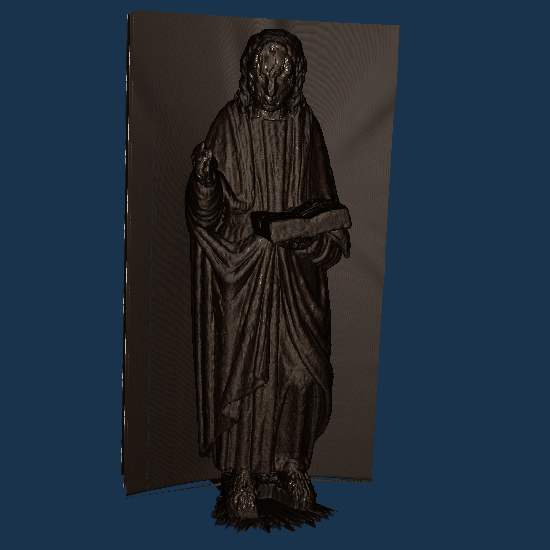
\includegraphics[width=5cm]{imagenes/primer_renderizado}
	\caption{Primer renderizado sobre la figura de San Juan Evangelista con una función de transferencia que no utilizaba la opacidad gradiente}
	\label{fig:primer_renderizado}
\end{figure}

Una vez comprobado que se estaba realizando bien el renderizado, se debía mejorar la función de transferencia. Para ello se creo una \textbf{barra de herramientas} (Figura \ref{fig:gui_inicial_tf}) con la que poder cambiar esta función de transferencia añadiendo puntos a ésta. Pese a no ser muy amigable para el usuario, era un primer prototipo que ayudaría a crear una función de transferencia con la que poder seguir trabajando.

\begin{figure}[H]
	\centering
	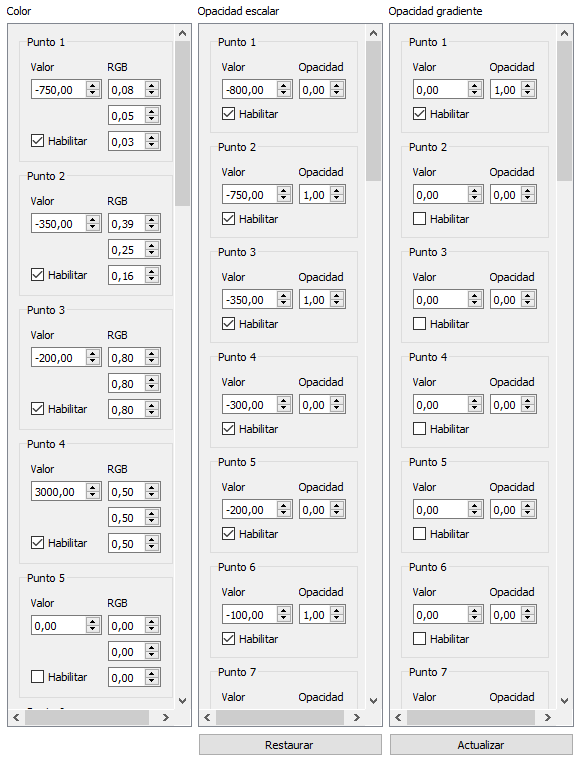
\includegraphics[width=7cm]{imagenes/gui_inicial_tf}
	\caption{Barra de herramientas con la que añadir y quitar puntos a la función de transferencia}
	\label{fig:gui_inicial_tf}
\end{figure}

\subsection{Generación de cortes}

Antes de mejorar la forma en la que se edita la función de transferencia se pasó a realizar una de las partes más importantes. La de la poder ver cortes de la figura. Para empezar se creó un nuevo \textit{widget} con el que se combinó lo implementado anteriormente para visualizar cortes (Figura \ref{fig:read_dicom_series_qt}). 

Pero de esta forma no se estaban generando cortes sino visualizando las propias imágenes con las que se reconstruía el volumen. La idea era poder \textbf{crear un corte en la figura dado por un plano arbitrario}. Para ello se hizo uso de \texttt{vtkImagePlaneWidget} modificando esta clase para que se renderizase el corte al mismo tiempo que se movía el plano. Este plano se conectaba con los datos del volumen (\texttt{vtkImageData}) para mostrar la salida en un \texttt{vtkImageViewer2} (Figura \ref{fig:primer_plano_de_corte}).

\begin{figure}[H]
	\centering
	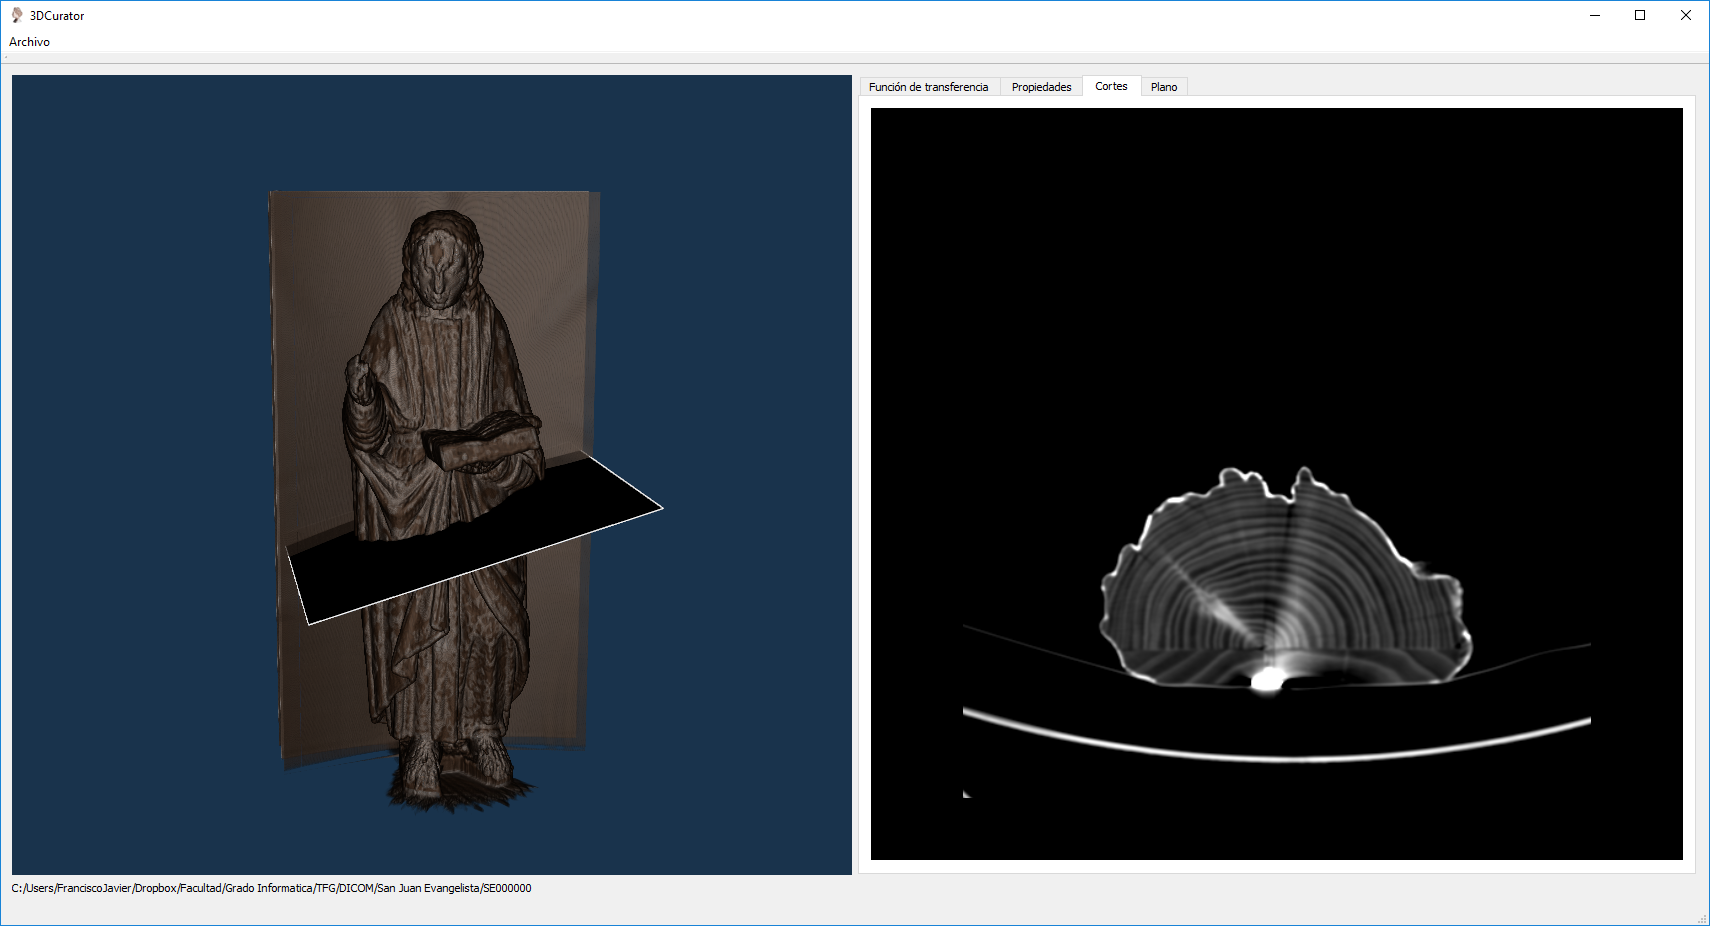
\includegraphics[width=12cm]{imagenes/primer_plano_de_corte}
	\caption{Primera implementación del plano que corta la figura y renderiza el corte en otro \textit{widget}}
	\label{fig:primer_plano_de_corte}
\end{figure}

Resultó sencillo añadir a continuación mejoras a este plano, como colocarlo en \textbf{posiciones por defecto} (axial, coronal y sagital) y visualizar la salida con el \textbf{mismo color que la función de transferencia}.

Además se reescribieron métodos de eventos de ratón para eliminar los innecesarios que ya traían las clases de VTK.

\subsection{Guardar imágenes}

Otra funcionalidad básica era la de poder \textbf{guardar imágenes de ambos visores}. VTK ofrece con las distintas subclases de \texttt{vtkImageWriter} una serie de clases con las que exportar imágenes en distintos formatos. Se han utilizado tanto \texttt{vtkJPEGWriter} como \texttt{vtkPNGWriter} para darle al usuario la posibilidad de guardar la imagen tanto en JPG como en PNG. 

\subsection{Editar función de transferencia}

Con el software cada vez más completo, era el momento de mejorar la \textbf{edición de función de transferencia}. La implementación anterior (Figura \ref{fig:gui_inicial_tf}) no ofrecía retroalimentación visual al usuario de cómo era la curva de la función o la paleta de colores. Además, añadir y editar puntos era un trabajo tedioso.

Resultaba imprescindible cambiarlo y la forma más cómoda de editar la función era trabajar sobre la misma. Es decir, \textbf{mostrar la función en una gráfica} con cada uno de sus puntos y poder mover, añadir o borrarlos interactuando directamente con la gráfica.

Explorando entre las clases que proporcionaba VTK se encontraron:

\begin{itemize}
	\item \texttt{vtkColorTransferFunctionItem}: Muestra la función de transferencia de color como un \texttt{vtkPlot} que se puede añadir a una \texttt{vtkChartXY}.
	\item \texttt{vtkPiecewiseFunctionItem}: Muestra la función de transferencia de opacidad como un \texttt{vtkPlot} que se puede añadir a una \texttt{vtkChartXY}.
	\item \texttt{vtkColorTransferControlPointsItem}: Muestra y permite modificar los puntos de la función de transferencia de color como un \texttt{vtkPlot} que se puede añadir a una \texttt{vtkChartXY}.
	\item \texttt{vtkPiecewiseControlPointsItem}: Muestra y permite modificar los puntos de la función de transferencia de opacidad como un \texttt{vtkPlot} que se puede añadir a una \texttt{vtkChartXY}.
\end{itemize}

No obstante, había que reescribir algunos métodos de estas clases para poder adaptarlas al software. Había que eliminar algunos eventos innecesarios y agregar nuevas acciones a otros como volver a renderizar el volumen cada vez que se cambie algún punto.

Llevar a cabo este trabajo fue bastante costoso pero finalmente se logró proporcionar al usuario una interfaz gráfica para editar la función de transferencia intuitiva y fácil de utilizar (Figura \ref{fig:gui_final_tf}).

\begin{figure}[H]
	\centering
	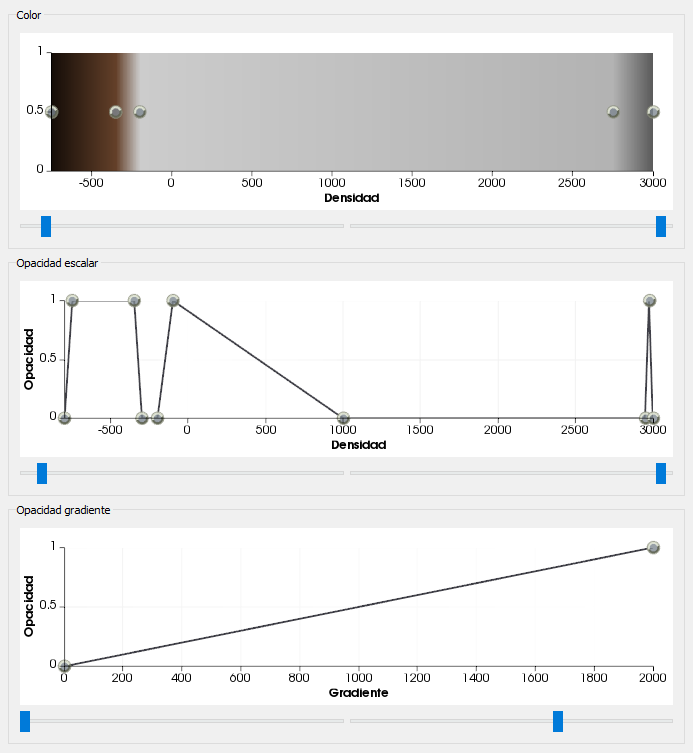
\includegraphics[width=10cm]{imagenes/gui_final_tf}
	\caption{Interfaz para editar la función de transferencia}
	\label{fig:gui_final_tf}
\end{figure}

\subsection{Importar y exportar función de transferencia}

Con la nueva interfaz iba a resultar sencillo crear una batería de funciones de transferencia, por tanto, llegó el momento de almacenarlas de alguna forma para luego poder usarlas.

Para esto se decidió utilizar XML almacenándolas con un formato en el que el software pudiese exportar e importarlas (Código \ref{code:xmlschema}).

\lstinputlisting[caption={Descripción de formato XML utilizado usando XML Schema}, label=code:xmlschema, style=XML]{misc/tf-xmlschema.xml}

Por ejemplo, la función de transferencia principal utilizada en este formato XML sería la siguiente (Código \ref{code:xmltf})

\lstinputlisting[caption={Ejemplo de función de transferencia en el formato XML descrito}, label=code:xmltf, style=XML]{misc/ct-woodsculpture.xml}

Para poder \textbf{gestionar estos ficheros}, se decidió utilizar una librería. Había muchas opciones, pero lo que se quería gestionar era bastante básico por lo que utilizar una demasiado compleja podría resultar contraproducente ya que se tardaría bastante tiempo en aprender a utilizarla.

Finalmente se optó por \textbf{Boost}, una librería muy extensa que cuenta con un pequeño gestor de ficheros XML. 

A partir de un fichero XML, Boost transforma la información a un \texttt{struct} en forma de árbol de forma que luego se puede recorrer fácilmente obteniendo la información deseada.

\subsection{Realizar medida}

Una de las primeras ideas que surgieron para añadir al software era la de poder realizar medidas. Pues esto podría resultar de mucha utilidad para los restauradores.

En poco tiempo se consiguió, gracias a la clase \texttt{vtkDistanceWidget} añadir una regla con la que \textbf{realizar medidas} (Figura \ref{fig:primera_regla}).

\begin{figure}[H]
	\centering
	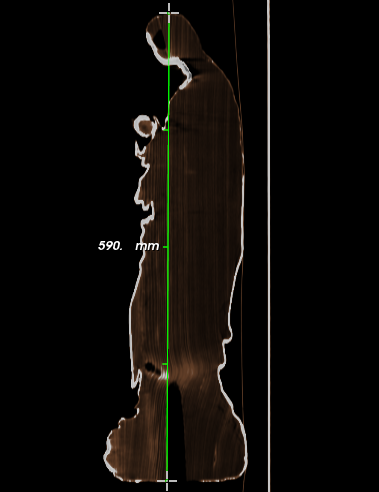
\includegraphics[width=8cm]{imagenes/primera_regla}
	\caption{Primera implementación de regla para medir. Solo se podía utilizar una en el visor de cortes}
	\label{fig:primera_regla}
\end{figure}

Lo ideal sería poder añadir más de una regla, pero antes de llevar esta mejora a cabo, se decidió pasar a otra quizás más importante.

\subsection{Borrar partes innecesarias}

Al hacer \textit{ray casting} se mapean los datos de la imagen en valores de color y opacidad gracias a la función de transferencia. Esto hace que se puedan diferenciar distintos materiales. Pero hay materiales con compuestos similares que pueden aparecer pues se encontraban en el escáner a la hora de realizarse la tomografía.

Hablo de \textbf{la camilla donde está apoyada la figura} que tiene zonas en las que hay un material con una densidad similar al estuco y otra con uno similar a la madera. Por lo que, al visualizarse, aparecen. Aunque no tienen nada que ver con la figura. Y no solo sobran, también molestan pues en el caso de una capa de la camilla, impide ver la figura a las espaldas (Figura \ref{fig:necesario_borrar}).

\begin{figure}[H]
	\centering
	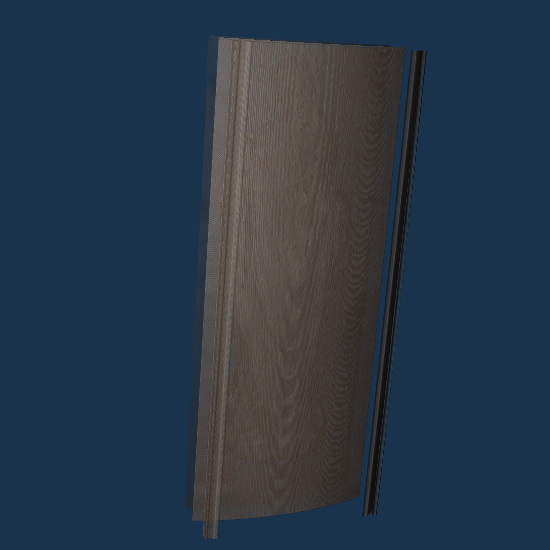
\includegraphics[width=8cm]{imagenes/necesario_borrar}
	\caption{La camilla tapa la espalda de la figura e impide verla}
	\label{fig:necesario_borrar}
\end{figure}

Es por tanto necesario proveer al software de una herramienta para poder \textbf{borrar estas partes}.

En un principio se pensó hacer un borrado en el que a partir de un punto seleccionado por el usuario, se \textbf{extendiese en 3D} comprobando si alguno de los puntos de alrededor tiene un valor similar para seguir extendiéndose recursivamente. Pero la camilla pegada a la figura tiene zonas donde las zonas de la camilla y la figura tienen un valor muy similar y esto provocaría que borrase en el interior de la figura.

La segunda capa de camilla, la más gruesa con valores de estuco (puede verse más blanca en las imágenes), está separada de la figura por un material con valores cercanos a los del aire y que, por tanto, no se muestran.

Esta situación hizo que se cambiase un poco el planteamiento y se borrase no por zonas con valor parecido sino por \textit{islas}. Entendiendo isla como una zona separada de las demás.

Se empezó a implementar el \textbf{algoritmo recursivo} descrito anteriormente, pero usando una pila de puntos a analizar en un bucle que continuase hasta que estuviese vacía en lugar de usar recursividad como tal pues podría agotar la pila de llamadas a funciones.

Sin embargo esto no solucionaba los problemas con el hardware porque, aunque no se agotase la pila de llamadas, la pila de puntos que se utilizaba se hacía demasiado grande. Tanto que agotaba la memoria utilizada por el programa.

Era necesario hacer un cambio y se pasó de extenderse en 3D a extenderse en 2D imagen por imagen. Pasando de introducir 26 puntos en cada iteración a 8 con un tamaño total de $ res_{x} \times res_{y} $ que hace que las coordenadas de una imagen de $ 1024px \times 1024px $ tenga espacio de sobra en la memoria de la pila sin desbordarse.

Este cambio no solo era más óptimo en cuanto a utilización de memoria, sino que resultaba bastante más rápido. Y, aunque en ocasiones, no borre la isla con un solo click, el proceso de borrado tarda escasos segundos (Código \ref{code:pseudo_delete}).

\begin{lstlisting}[style=C, label=code:pseudo_delete, caption={Pseudocódigo del borrado}]
void deletByImages(data, point, bounds) {
	deleteImage(data, point, bounds)
	z = point.z + 1
	while (z < bounds.z.max) {
		point.z = z
		deleteImage(data, point, bounds)
		z++
	}
	z = point.z - 1
	while (z >= bounds.z.min) {
		point.z = z
		deleteImage(data, point, bounds)
		z--
	}
}

void deleteImage(data, point, bounds) {
	z = point.z
	xy = {point.x, point.y}
	if (data(point) < AIR_HU) {
		point = searchInitialVoxel(data, point, bounds)
	}
	stack.push(xy)
	while (!stack.empty()) {
		xy = stack.pop()
		if (isInside(xy, bounds)) {
			point = {xy.x, xy.y, z}
			if (data(point) >= MIN_AIR) {
				data(point) = AIR_HU
				stack.push(pointsAround(point))
			}
		}
	}
}
\end{lstlisting}

Gracias a este algoritmo de borrado se puede eliminar fácil y rápidamente la camilla que no está pegada a la figura y, al ser la capa que está pegada muy fina y tener activada la opacidad gradiente, se puede ver las espaldas de la figura a diferencia de antes (Figura \ref{fig:camilla_borrada}).

\begin{figure}[H]
	\centering
	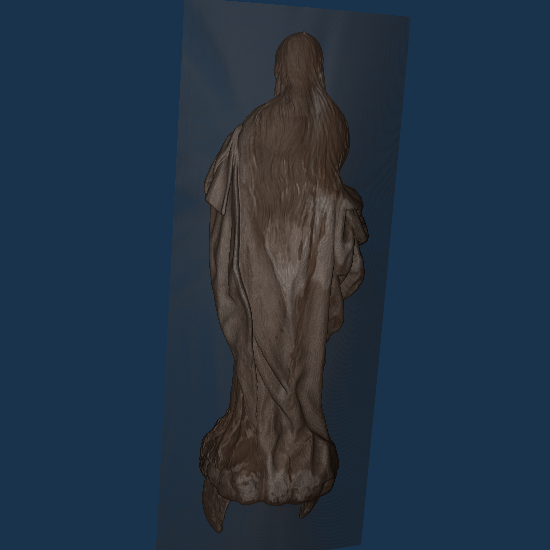
\includegraphics[width=8cm]{imagenes/camilla_borrada}
	\caption{La camilla ha sido eliminada y permite ver la espalda a diferencia de antes (Figura \ref{fig:necesario_borrar})}
	\label{fig:camilla_borrada}
\end{figure}

No obstante, y aunque esta capa que se sigue viendo no molesta tanto, a la hora de realizar el escáner podría resultar útil colocar un material que se sepa que tiene un valor de densidad similar al aire entre la figura y la camilla para que así pueda ser borrada por completa la camilla.

\subsection{Exportar malla de triángulos}

Una de las últimas ideas de funcionalidad a introducir en el software es la de la \textbf{generación de una malla de triángulos} del modelo que pudiese ser exportada en formato STL.

Para ello, como se avanzó con anterioridad, se utiliza la técnica de \textit{marching cubes} y la clase \texttt{vtkMarchingCubes} que VTK proporciona para ello.

Por lo que se introduce otro \textit{widget} en la aplicación para visualizar la malla generada a partir de un valor de isosuperficie dado por el usuario.

De esta forma se puede obtener, por ejemplo, un modelo de los clavos de una figura \ref{fig:malla_clavos} que luego podrían imprimirse con una impresora 3D.

\begin{figure}[H]
	\centering
	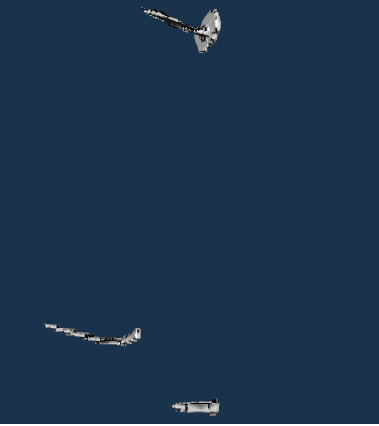
\includegraphics[width=8cm]{imagenes/malla_clavos}
	\caption{Malla generada con un valor de isosuperficie de 2976 HU para poder extraer los clavos}
	\label{fig:malla_clavos}
\end{figure}

\subsection{Mostrar valor de densidad}

Al empezar a crear la función de transferencia, ya se comentó la utilización de otro software para comprobar \textbf{el valor escalar de cada pixel} de la imagen para poder ver entre qué valores se movía cada material. Es por ello que pareció interesante añadir en la interfaz esta información.

Por lo que, como última idea de mejora, y aprovechando lo aprendido de los \textit{pickers} durante la implementación del borrado, se añadió a la interfaz una etiqueta donde se muestra el valor del pixel sobre el que el ratón está posicionado.

\subsection{Realizar varias medidas}

Dada por finalizada la lluvia de ideas que añadir como mejoras, había que realizar todo aquello que se decidió implementar más adelante.

Hablo principalmente de la \textbf{gestión de reglas para realizar varias medidas} en cualquiera de los dos visores principales. Para ello había que dotar a la interfaz de un cuadro con las reglas con opciones para añadir, eliminar y habilitar o deshabilitar.

Dado que contaba con la experiencia justa con Qt, se realizó en primer lugar la gestión de elementos de la interfaz para poder posteriormente mapear cada item de las cajas a un \texttt{vtkDistanceWidget} distinto.

\begin{figure}[H]
	\centering
	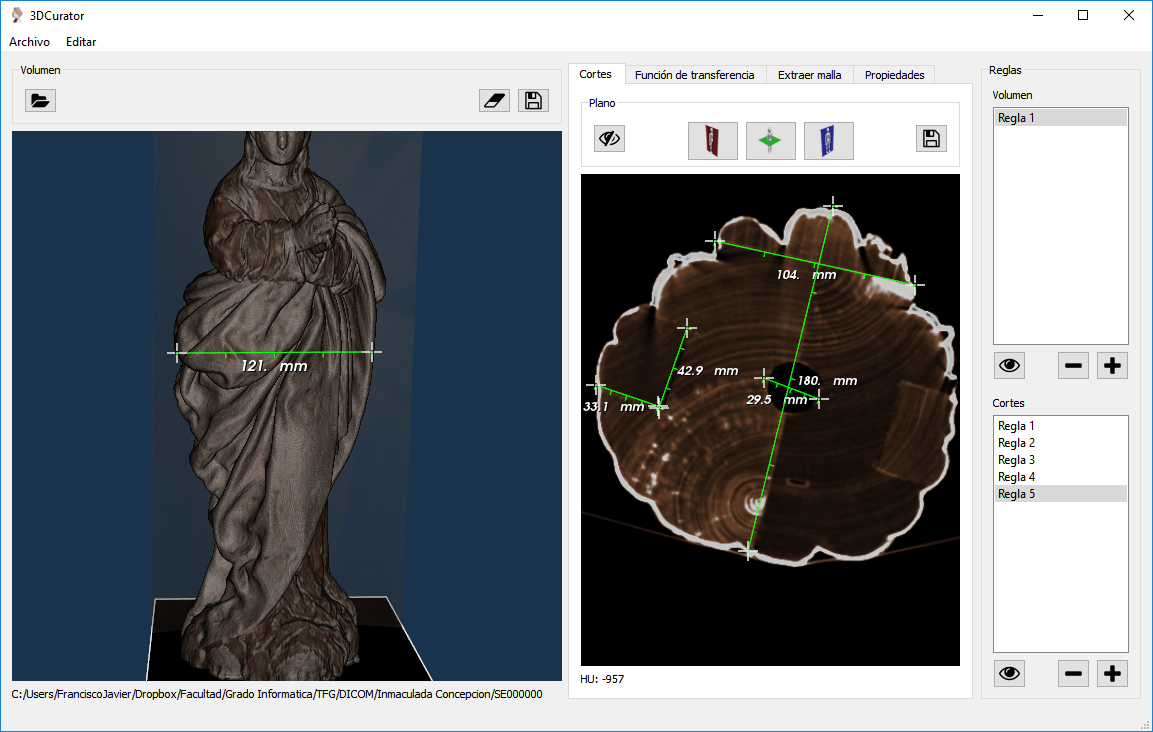
\includegraphics[width=12cm]{imagenes/varias_reglas}
	\caption{A la derecha, barra de las reglas y en los visores cada una de ellas midiendo algo distinto}
	\label{fig:varias_reglas}
\end{figure}

\subsection{Cambiar color de fondo de los visores}

Una de las primeras ideas que se pensaron fue la de poder permitir cambiar al usuario el \textbf{color de fondo de los \textit{widget}} donde se visualizan tanto el volumen como la malla generada. Pero no se realizó hasta al final pues había cosas más importantes que implementar.

Con esta pequeña mejora junto a otras menores en la interfaz, se dio por terminada la fase de desarrollo del software. Cumpliendo los requisitos iniciales y añadiendo múltiples mejoras que han acabado formando un software bastante completo pero al mismo tiempo sencillo de utilizar.

\subsection{Web de presentación}

Una vez acabado el software y creado un instalador para Windows, aprovechando la funcionalidad de \textit{GitHub Pages} que permite alojar gratuitamente una web para un repositorio, se creó una \textbf{web estática} en la que presentar el software y proporcionar un enlace de descarga, así como enlaces para poder contactar conmigo. La dirección a ésta es: \href{http://fblupi.github.io/3DCurator/}{http://fblupi.github.io/3DCurator/}.